%==========================================================================
% BEGIN #6 - IMPLEMENTAÇÃO
% Descrição detalhada do processo de implementação realizado, referindo as opções de desenvolvimento que foram adotadas e as decisões tomadas. Apresentação da estrutura da aplicação desenvolvida e de cada um dos seus serviços, ilustrando um ou dois processos que tenham sido implementados. Reportar o desempenho da aplicação e, em particular, de cada um dos serviços implementados. 

% 1) Apresentação e descrição do processo de implementação realizado.

% 2) Apresentação da aplicação e explicação dos serviços implementados.

% 3) Analise e avaliação da aplicação desenvolvida.

%==========================================================================


\chapter{Implementação da Aplicação}
    
    \section{Descrição do Processo de Implementação}

            O arranque da fase de implementação inaugurou-se com um debate sobre qual \textit{framework} de desenvolvimento enquadrada no \textit{ASP.NET} se via mais adequado tanto para o contexto em mão e para a equipa. Dada a preferência por linguagens já familiares, escolheu-se o \textit{Blazor} ao invés do mais ubíquo ASP.NET Core MVC, por permitir a escrita em \textit{C\#} para todas as camadas do programa.   
                
        \newpage
        \subsection{\textit{Back End}}

            \subsubsection{Tecnologias/Ferramentas Utilizadas}
                    Dado o contexto de .NET, foi decidido o recurso ao SQL Server como gestor de base de dados, por ser a opção mais comum e à responsabilidade da mesma Microsoft, o que induz maior compatibilidade, melhor apoio técnico e mais facilidade na potencial integração de recém-contratados para mantuenção do sistema no futuro. 
        
            \subsubsection{Acesso a Dados}
                % Estratégia de Acesso a Dados (Database-First/DAOs vs Code-First/Entity Framework)
                    A estratégia de acesso a dados foi alvo de ponderação sobre o uso de \textit{Entity Framework Core (EFCore)}, que implica a estipulação \textit{a priori} de modelos lógicos suportados por parâmetros que permitem a inferência automática dunm contexto de base de dados, controladores e de páginas genéricas para ponto de partida da camada de apresentação. Este paradigma denomina-se "código primeiro". No entanto, o facto de já haver tabelas definidas em antemão fez com que se utilizasse antes o método "base de dados primeiro", com modelos feitos manualmente. Os modelos são então instanciados via objetos de acesso a dados (DAOs), que abstraem as interações necessárias com a base de dados.

                % Queries de Criação das Tabelas
                    Foi elaborado o \textit{script} visto à frente para a criação da base de dados do sistema.
                    \newpage
                    \lstinputlisting[breaklines,basicstyle=\ttfamily\tiny,label=lst:sqlcreatedb]{code/sqlcreatedb.sql}
                % Definição de Objetos de Acesso a Dados (DAOs)
                    O programa acede à base de dados graças à biblioteca de classes \texttt{DataAccess} adicionada como dependência, que define \texttt{[Order|Piece|Set|User]DAO} como DAOs. São parecidos no sentido em que todos disponibilizam métodos para interação com a base de dados, mas diferem em termos da temática para qual se orientam. Deste modo, há um maior grau de separação de matérias no código, tornando-o mais organizado. Ao ser do interesse a certo método na camada de negócio interagir com a base de dados por um motivo primariamente referente a encomendas, deve partir de \texttt{OrderDAO}. Esta fragmentação é cada vez mais útil à medida que o sistema cresce em complexidade de modelos e subsistemas.
                
                    Estes DAOs comunicam com a base de dados graças à classe \texttt{DatabaseAccess}, que fornece a \textit{string} de conexão.
            \newpage
            \subsubsection{Lógica de Negócio}
            
                % Definição de Modelos de Dados (Com base no domínio estabelecido no capítulo 3) 
                    Foram definidos os modelos de dados na biblioteca de classes \texttt{Models} adicionada como dependência, servindo a função não só de entidades representantes dos dados mas também de modelos de apresentação (\textit{view models}). É de frisar que, no contexto duma aplicação de maior escala, seria preferível o estabelecimento de modelos de apresentação completamente separados dos modelos de dados, pois é uma prática promotora da assincronicidade de desenvolvimento que permite aos encarregados pela camada apresentativa não depender de potenciais alterações feitas por programadores mais abaixo na cadeia.
                    \lstinputlisting[breaklines,basicstyle=\ttfamily\tiny,label=lst:models]{code/Models.cs}
                    % Piece, Set, Order, User    
                
                % Lógica em Páginas Razor
                    \newpage
                    As páginas \textit{Razor} possibilitaram a implementação de lógica de negócio em conjunto com o formato HTML das páginas. Isto resultou num certo acoplamento de código que, num caso de maior escala, seria preferível de abstrair para subsistemas, assim conseguindo potencialmente fazer do \textit{back end} uma mera interface de programação (API) e flexivelmente substituir o \textit{front end} por completo se necessário.

                    Sendo um programa de gestão, a maioria dos requisitos assentam na visualização de dados. Tal torna a camada de lógica de negócio relativamente "fina" e, com isso em mente, tomou-se a decisão de fazer chamadas diretamente das páginas Razor aos DAOs. A título de exemplo, observe-se o excerto de código abaixo, incluído na página para pedido de reposição manual. O método \texttt{Submit} é chamado quando o botão de igual nome é carregado.
                    
                    \lstinputlisting[breaklines,basicstyle=\ttfamily\tiny, label=lst:restockrequest]{code/RestockRequest.cs}
                    
        \newpage
        \subsection{\textit{Front End}}

            \subsubsection{Tecnologias/Ferramentas Utilizadas}
                Graças ao uso de componentes Blazor e páginas Razor no geral, apenas foi necessária a utilização de HTML e CSS para dar à aplicação um estilo próprio e com um grau de fidelidade para com os esboços da interface elaborados na etapa anterior.
                
            \subsubsection{Mapa de Páginas}
                Observe-se um mapa de navegação pela aplicação. Nada é acessível ao utilizador antes de se autenticar, pelo que depois disso é-lhe apenas impedido o acesso à edição de inventário até à inserção duma senha administrativa válida.

                \begin{figure}[h!]
                    \centering
                    \includegraphics[width=0.99\linewidth, frame]{images/Site/sitemap.pdf}
                    \caption{Mapa de Páginas}
                    \label{fig:sitemap}
                \end{figure}
                
    \newpage
    \section{Serviços e Funcionamento} % Screenshots da app ficam nesta secção
        
            \subsection{Serviços Relativos a Utilizadores}
                \subsubsection{Sessões de Utilizador}

                            \begin{figure}[h!]
                                \centering
                                \includegraphics[width=0.8\linewidth, frame]{images/Site/Login.pdf}
                                \caption{Página de início de sessão}
                                \label{fig:Página de login}
                            \end{figure}

                            \begin{figure}[h!]
                                \centering
                                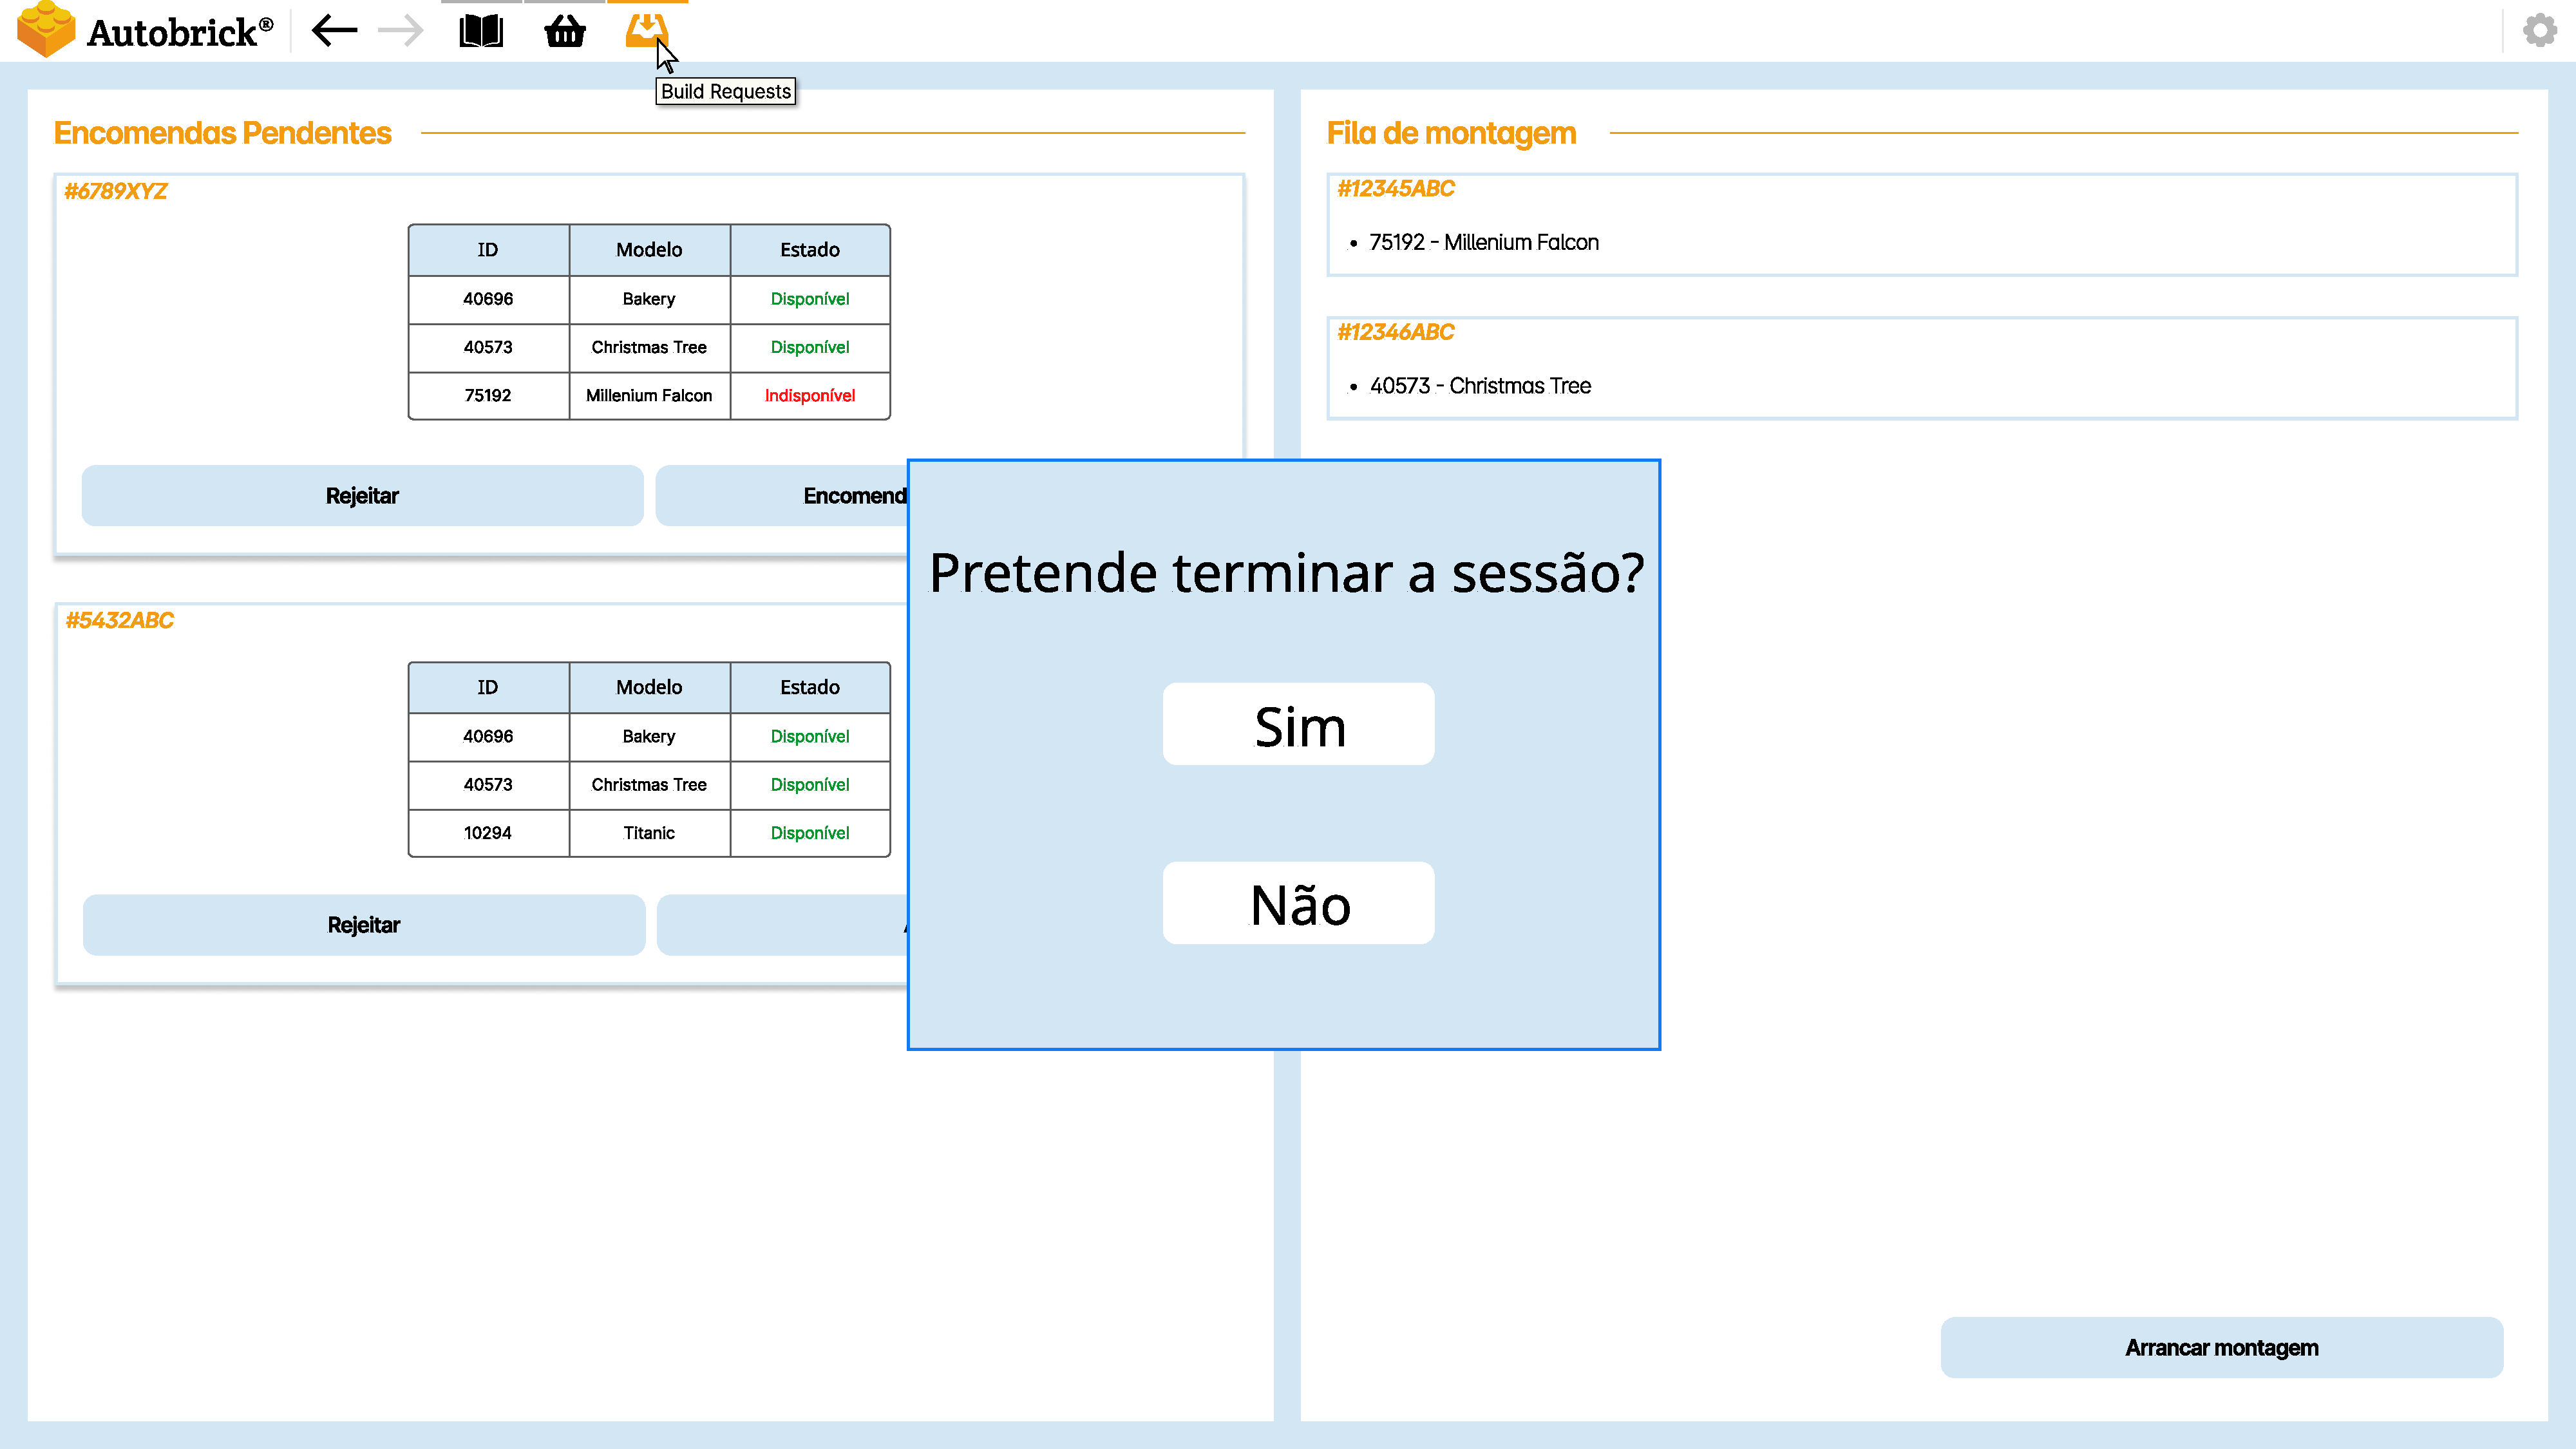
\includegraphics[width=0.8\linewidth, frame]{images/Site/Logout.pdf}
                                \caption{Página de término de sessão}
                                \label{fig:Página de logout}
                            \end{figure}

                    Estsa são as páginas vistas antes do início de sessão no sistema e após o término da mesma (ver requisitos 2.2.2/2.2.3). O que é inserido nos campos é submetido a verificação contra as credenciais armazenadas na base de dados (ver 2.2.1). Não é percetível, mas note-se adicionalmente que a sessão é guardada em cookie de autenticação com 30 minutos de validade. Assim, se não se terminar a sessão, é possível fechar e voltar a abrir o sistema dentro desse espaço de tempo sem precisar de iniciar sessão de novo.

                    % Satisfaz Reqs...
                        % 2.2.1 (teste de validade de senha)
                        % 2.2.2/3 (início/término de sessão)
                        % 2.2.4 (detalhes da conta, ao ver nome na barra superior)
                    % Explicar mantimento de sessão via cookie de autenticação com 30 minutos de vida (ver Program.cs) 

            \clearpage
            \subsection{Serviços Relativos a Encomendas}
                \subsubsection{Consultar Encomendas Pendentes}

                            \begin{figure}[h!]
                                \centering
                                \includegraphics[width=0.8\linewidth, frame]{images/Site/Pending Orders.pdf}
                                \caption{Página de encomendas pendentes}
                                \label{fig:Página de encomendas pendentes}
                            \end{figure}

                    Nesta página o utilizador pode consultar todas as encomendas pendentes (ver 2.3.1) bem como analisar a sua viablidade (ver 2.3.2). Após analisada ele pode adicioná-la à fila de montagem (ver 2.3.4), recusar (ver 2.3.3) ou encomendar as peças que não estão disponíveis tendo em conta todos os modelos que inclua (ver 2.4.3). Pode ainda consultar o seu nome de utilizador através da barra de navegação (ver 2.2.4).

                
                    % Satisfaz Reqs...
                        % 2.3.1 (consultar encomendas pendentes)
                        % 2.3.2 (viabilidade de encomenda pendente)
                        % 2.3.3 (recusar encomenda pendente)
                        % 2.3.4 (colocar encomenda pendente em fila)
                        % 2.4.3 (reposição automática com base em peças que faltem a encomenda)
                \subsubsection{Consultar Fila de Montagem de Encomendas}
                    
                    \begin{figure}[h!]
                        \centering
                        \includegraphics[width=0.8\linewidth, frame]{images/Site/Queued Orders.pdf}
                        \caption{Página de fila de montagem de encomendas}
                        \label{fig:Página de fila de montagem de encomendas}
                    \end{figure}

                    Esta página contem todas as encomendas que foram colocadas em fila de montagem (ver 2.3.5). Aqui o utilizador pode arrancar com a montagem de uma encomenda (ver 2.3.6) e posteriormente marcar essa encomenda como finalizada (ver 2.3.7).

                    % Satisfaz Reqs..
                        % 2.3.5 (consulta da fia de montagem)
                        % 2.3.6 (arrancar fila de montagem - simplificado para consulta de modelos intra-encomenda)
                        % 2.3.7 (confirmar montagem de modelo em encomenda - simplificado para finalização geral da encomenda)

            \subsection{Serviços Relativos a Modelos}
                \subsubsection{Consulta a Catálogo de Modelos} % 2.5.1 (consultar catálogo de modelos)

                    \begin{figure}[h!]
                        \centering
                        \includegraphics[width=0.8\linewidth, frame]{images/Site/Set Index.pdf}
                        \caption{Página de catálogo de modelos}
                        \label{fig:Página de catálogo de modelos}
                    \end{figure}

                    Nesta página está disponível uma lista com todos os modelos registados no sistema bem como a possibilidade de ver o manual de um modelo que pretender (ver 2.5.2 e 2.5.3)

                    
                \subsubsection{Visualizar Sequência de Montagem de Modelo}
                    
                    \begin{figure}[h!]
                        \centering
                        \includegraphics[width=0.8\linewidth, frame]{images/Site/Manual.pdf}
                        \caption{Página com sequência de montagem de modelo}
                        \label{fig:Página de fila de montagem de encomendas}
                    \end{figure}

                    Aqui temos a página do manual do respetivo modelo onde o utilizador pode andar para a frente e para trás no manual ou voltar à lista de modelos.
                    
                    % Satisfaz Reqs...
                        % 2.5.2 (visualizar montagem de modelo)
                        % 2.5.3 (existência de manual para modelo // nao-funcional)

            \subsection{Serviços Relativos ao Inventário}
                
                \subsubsection{Consulta a Inventário de Peças} % Req. 2.4.1
                    
                    \begin{figure}[h!]
                        \centering
                        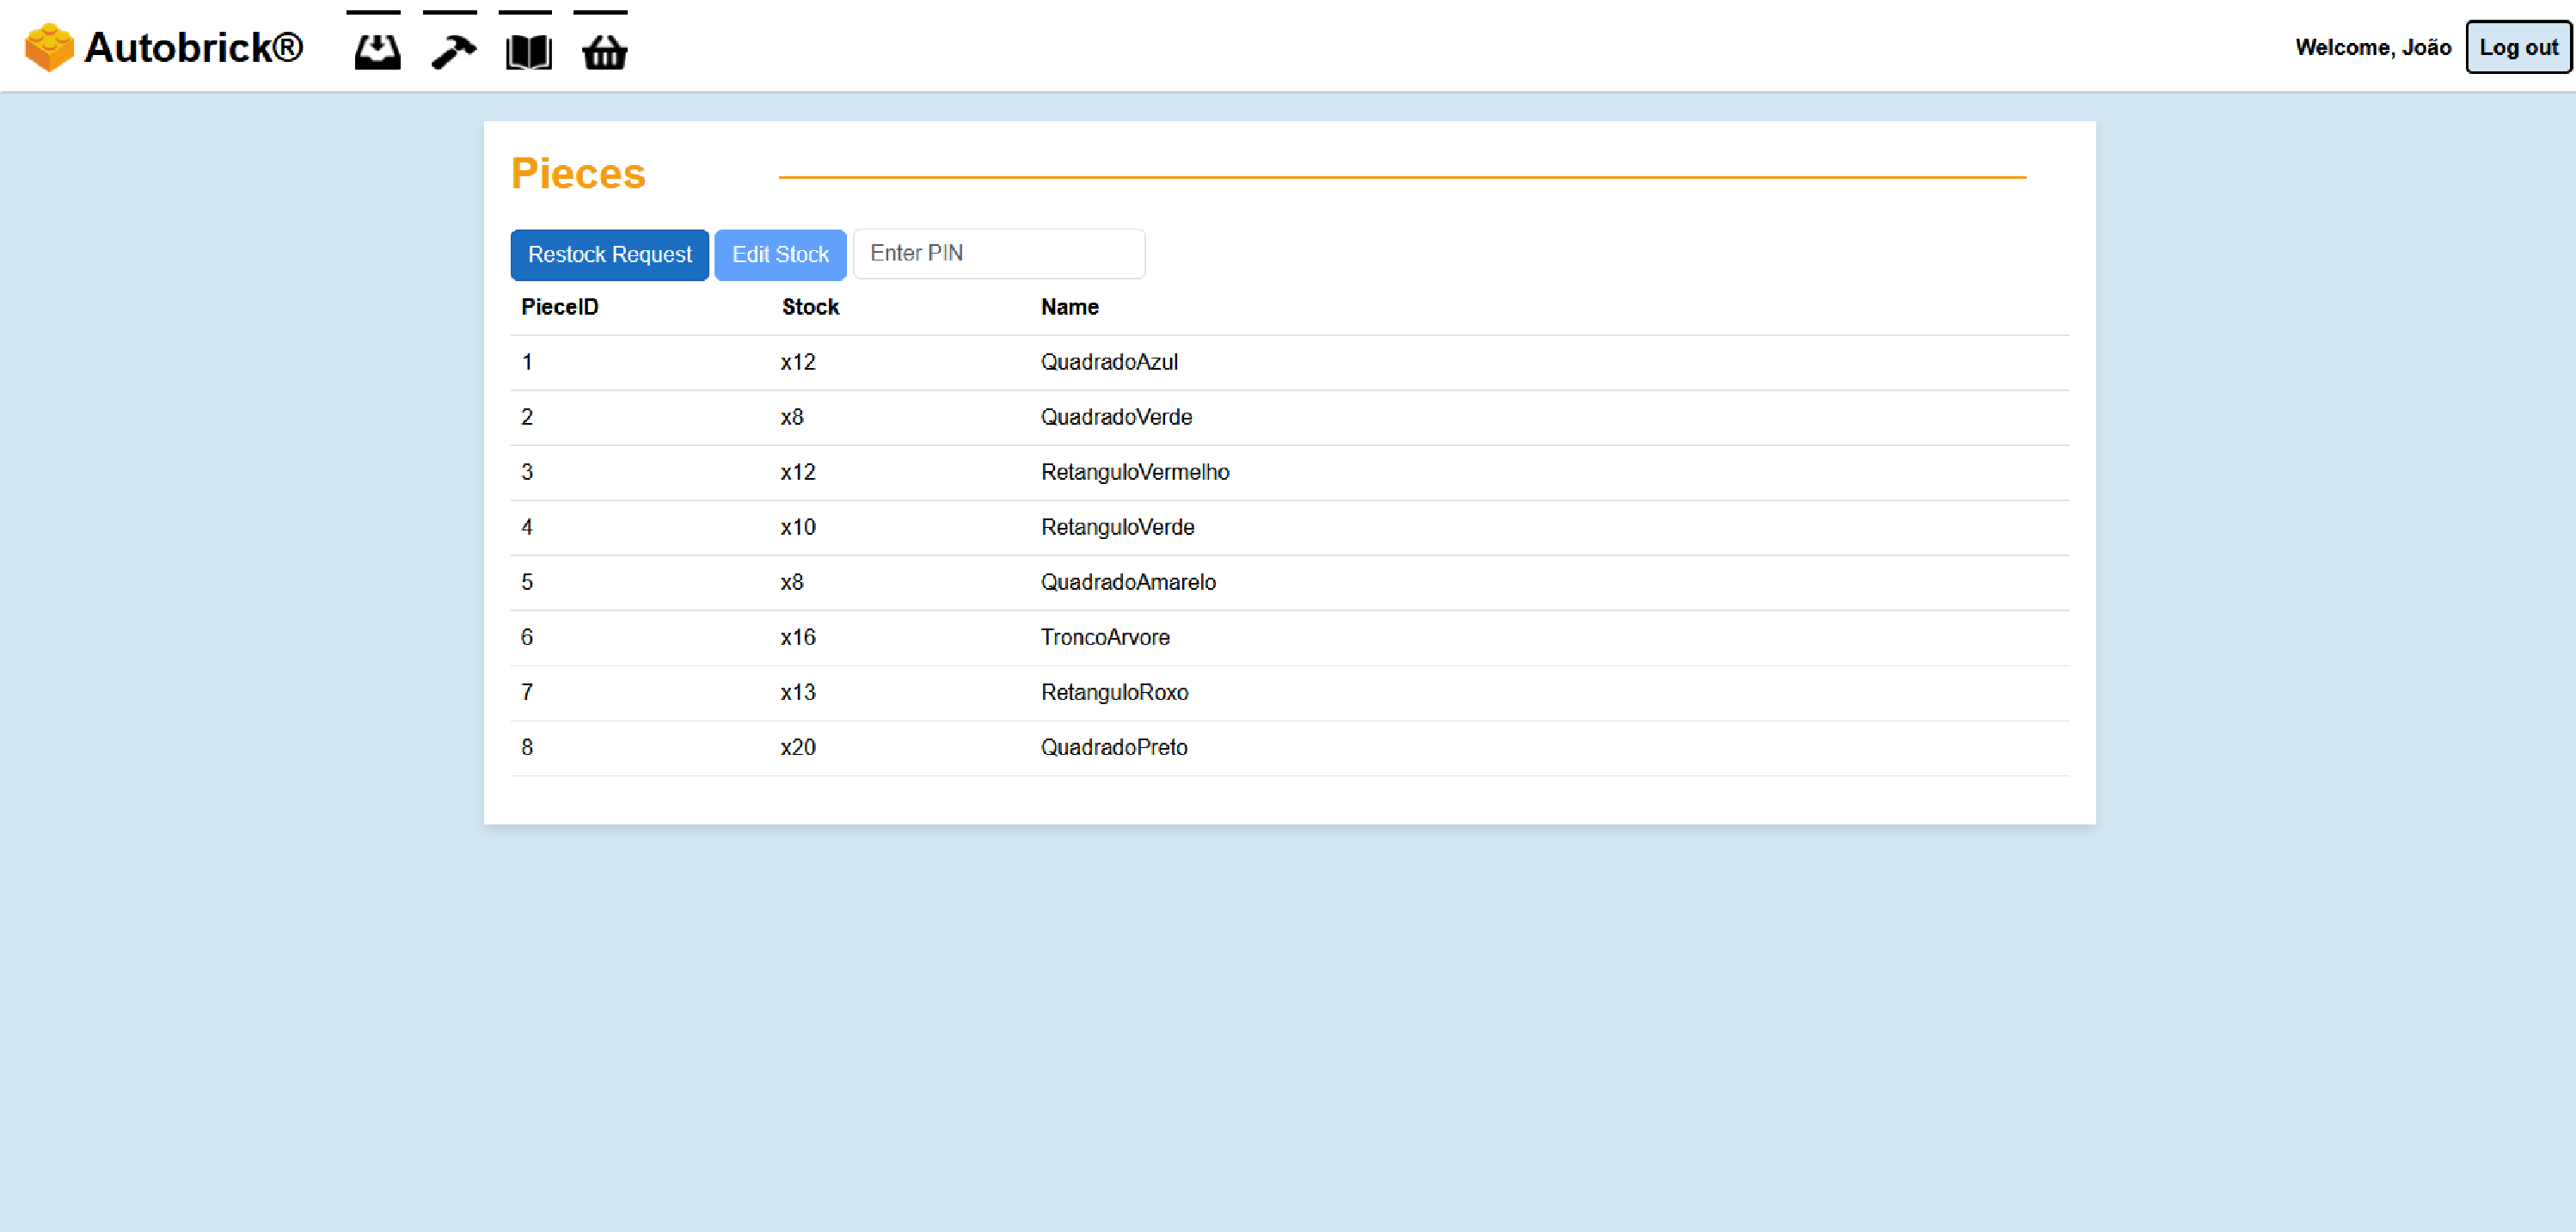
\includegraphics[width=0.8\linewidth, frame]{images/Site/Inventory.pdf}
                        \caption{Página de inventário de peças}
                        \label{fig:Página de inventário}
                    \end{figure}

                    A página para consulta do inventário (ver requisito 2.4.1) apresenta todas as peças cujas quantidades disponíveis sejam não-nulas. É a partir daqui que se tem acesso à página para pedido de reposição e, após inserção dum código administrativo válido, à página de edição do inventário atual.
                
                \subsubsection{Pedido de Reposição Manual de Inventário} % Req 2.4.2 

                    \begin{figure}[h!]
                        \centering
                        \includegraphics[width=0.8\linewidth, frame]{images/Site/Restock.pdf}
                        \caption{Página de pedido de reposição de inventário}
                        \label{fig:Página de pedido de reposição de inventário}
                    \end{figure}

                    A página de pedido de reposição manual está disposta de modo a que todos os valores inseridos nos campos causem incrementação aos atuais valores de quantidade unitária nas correspondentes peças ao pressionar o botão \textit{Submit}.
                
                \subsubsection{(Administrativo) Editar Quantidades em Inventário} % Req 2.4.4

                    \begin{figure}[h!]
                        \centering
                        \includegraphics[width=0.8\linewidth, frame]{images/Site/EditStock.pdf}
                        \caption{Página de edição das quantidades em inventário}
                        \label{fig:Página de edição das quantidades em inventário}
                    \end{figure}    

                    Esta página apenas é acessível com uma chave de administrador e dá acesso à manipulação manual do inventário (ver 2.4.4). Após a confirmação, todos os valores inseridos irão sustituir aqueles que estavam previamente registados na página de stock.
        
    \newpage
    \section{Análise e Avaliação de Desempenho}

        \subsection{No Acesso a Dados}
        
        Confronto da implementação com os princípios ACID:
        \begin{itemize}
            \item Atomicidade: os métodods dos DAOs estão escritos de forma a haver rollback se qualquer exceção ocorrer.
            \item Consistência: qualquer das alterações à base de dados está estabelecida de modo a preservar integridade referencial. isto é especialmente crítico na rejeição de encomendas, dada a existência da tabela de junção entre uma encomenda e um modelo.
            \item Isolamento: não aplicável, pois a aplicação não recorre a programação concorrente.
            \item Durabilidade - não se fazem \textit{logs} ou registos de histórico de transações, algo que lhes acrescentaria resistência perante falhas de \textit{hardware}. No entanto, não há um mantimento prolongado de dados em memória volátil.
        \end{itemize}
        
        \subsection{Na Execução dos Serviços}
            
            O objetivo principal ao executar um serviço é que este seja o mais rápido e simples possível para o utilizador devido ao seu público-alvo e local de aplicação. A aplicação apresenta ao uma página de log in que permite ao mesmo autenticar-se para iniciar o trabalho. Ao utilizar a aplicação no contexto de aquisição de encomendas, a mesma garante que em tempo real o utilizador escolha que encomendas pretende efetuar, e em caso de ser necessário efetuar um pedido de restock para conseguir realizar a mesma. Permite controlar o inventário em tempo real, tendo atualização constante das peças que estão disponíveis para montagem e em caso de ser necessário o utilizador consegue efetuar um pedido de restock. No contexto de linha de montagem em si, o utilizador consegue ler o manual de instruções enquanto monta a peça, o mesmo permite passar a página e voltar para a anterior em tempo real. 
    
%==========================================================================
% END #6 - IMPLEMENTAÇÃO
%==========================================================================